\chapter{Example of a chapter}
\label{chap:example}

For the thesis format for BSU, here is an example Chapter.

\section{Summary}
 
This is an example of a Chapter. 

\section{Introduction}

We present an example of a Chapter

\section{\nobreak Example of a section}

This is an example of a Chapter, like in \citet{mythesis}. Let us
include Figure~\ref{fig:figure} from a paper we wrote a while back
\citep{scalesvanwijk01}. As you can see in examplechapter.tex, the
figure label is dynamic. This means that if you change the order of
the figures, or remove one, you will not have to renumber these by
hand.

By the way, in examplebib.bib are examples of most formats for your
bibliography. Another way of using natbib is like this: \cite[or][for
example]{mythesis}. For a complete overview of the features of the
natbib package for bibtex, see natbib.pdf in this directory.

\begin{figure}
  \center
  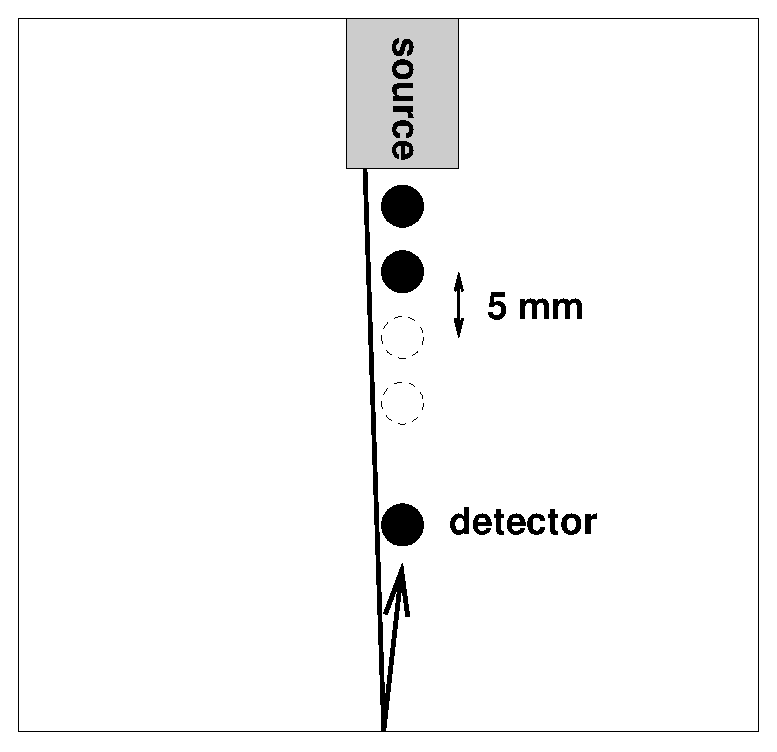
\includegraphics[width=7.5cm]{figures/setup}
  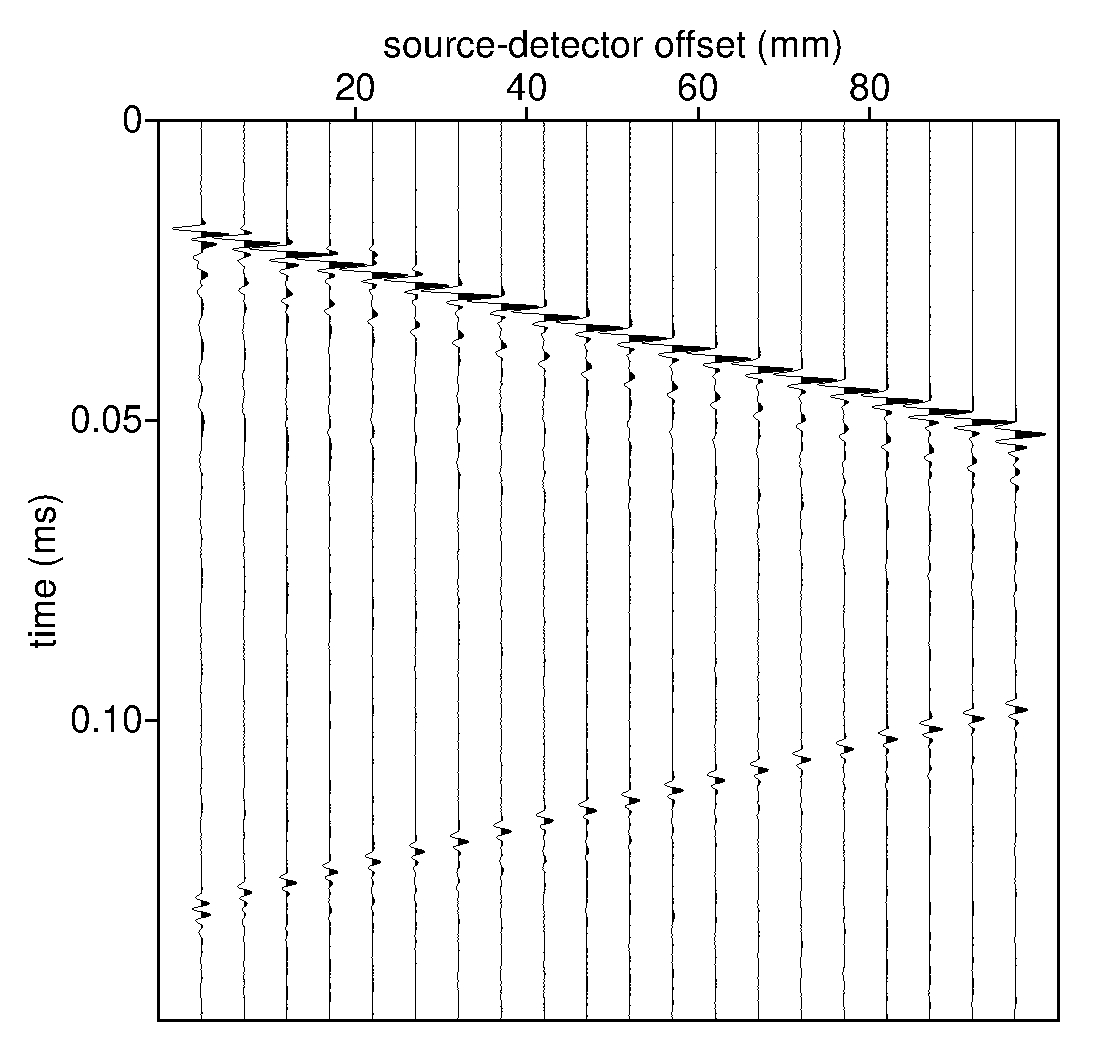
\includegraphics[width=7.5cm]{figures/exp0}
  \caption{Top-view of the experimental configuration (left) on the
    smooth face of aluminum.}
  \label{fig:figure}
\end{figure}

\subsection{Example of a subsection}

There are headings for chapters, sections, subsections and even
subsubsections:

\subsubsection{Appendices}

In Appendix~\ref{app:example} there is an example of an equation,
while 95\% confidence intervals for $\sigma$ are given in
Table~\ref{table:sigma}.
\begin{table}
  \caption{Approximate 95\% confidence intervals (in ms) for the true 
    standard deviation $\sigma=2.0$~ms of the VSP data. 
    The first column corresponds to the model-independent estimate, 
    the others are model-based estimates from the three different L-curves.} 
  \begin{center} 
    \begin{tabular}{|c|c|c|c|}\hline 
      $\sigma_\mu$  & $\sigma_I$ &$\sigma_{L}$  &$\sigma_{1/\lambda}$  \\
      \hline  
      2.02 $\pm$ 0.03 & 1.90 $\pm$ 0.03  & 1.92 $\pm$ 0.03 & 1.93 $\pm$ 0.03 
      \\ \hline 
    \end{tabular} 
    \label{table:sigma} 
  \end{center} 
\end{table} 

% usually, you'd let latex decide on the page breaks, but to create
% some pages for this template:
\newpage

more bla di bla (to create some more pages)


\subsection{Abbreviations}

\gls{ny}, \gls{la} and \gls{un} are abbreviations whereas
% \gls{angelsperarea}, \gls{numofangels} and \gls{areaofneedle} are part of the nomenclature
First use: \gls{svm}. Second use: \gls{svm}.



\newpage 

and a little more...


%%% Local Variables: 
%%% mode: latex
%%% TeX-master: "BSUmain"
%%% End: 
